\loai{Loại 1. Độ chênh lệch nhiệt độ}
\begin{vidu}
	\immini[thm]{Trung tâm nghiên cứu hạt nhân châu Âu (CERN) vận hành một máy gia tốc hạt lớn (Large Hadron Collider), trong đó có khoảng 9600 nam châm chuyên dụng để gia tốc proton. Các nam châm này được đặt trong môi trường lạnh đến $-271,2^\circ C$. Lấy $0^\circ C=273,15\ K$. Nhiệt độ $-271,2^\circ C$ tương ứng với giá trị nào theo thang Kelvin?
		\choice
		{$2,95\ K$}
		{$0\ K$}
		{\True $1,95\ K$}
		{$-1,95\ K$}}{
\includegraphics[width=4.6cm]{images/1144}}
		\loigiai{
			\begin{itemize}
				\item[A] Sai: Nhầm cộng $273,15$ và $-271,2$ thành $2,95$
				\item[B] Sai: $0\ K$ tương ứng với $-273,15^\circ C$, không đúng với $-271,2^\circ C$
				\item[C] Đúng: $K = -271,2 + 273,15 = 1,95$
				\item[D] Sai: Nhiệt độ Kelvin không có giá trị âm
			\end{itemize}
		}
\end{vidu}

\begin{vidu}
Thế giới từng ghi nhận sự thay đổi nhiệt độ rất lớn diễn ra ở Spearfish, South Dakota vào ngày 22/01/1943. Lúc $7h30$ sáng, nhiệt độ ngoài trời là $-20^\circ C$. Hai phút sau, nhiệt độ ngoài trời tăng lên đến $7,2^\circ C$. Tốc độ tăng nhiệt độ trung bình trong 2 phút đó là bao nhiêu Kelvin/giây (làm tròn kết quả  đến chữ số hàng phần trăm)?
	\shortans[oly]{ 0,23}
	\loigiai{
		\begin{itemize}
			\item Độ tăng nhiệt độ: $7,2+20=27,2^\circ$ hay 27,2 K.
			\item Tốc độ tăng nhiệt độ trung bình trong 2 phút là: $\dfrac{27,2}{2.60}\approx 0,23\ K/s$.
		\end{itemize}
	}
	\haidong{6}\end{vidu}
\loai{Loại 2: Quy đổi nhiệt độ Celsius – Kelvin}

\begin{vidu}
	Nhiệt độ mùa đông tại Thành phố New York (Mỹ) là 283 K. Ứng với nhiệt giai Celsius, nhiệt độ ở đó xấp xỉ là
	\choice
	{\True $10^\circ C$}
	{$-10^\circ C$}
	{$5^\circ C$}
	{$-5^\circ C$}
	\loigiai{
		Để chuyển từ thang Kelvin (K) sang thang Celsius ($^\circ C$), ta dùng công thức:
		\[ t_C = T_K - 273 \]
		Cụ thể:
		\[ t_C = 283 - 273 = 10^\circ C \]
	}
	\haidong{4}\end{vidu}

\begin{vidu}
	Theo bản tin thời tiết phát lúc 19h50 ngày 27/02/2022 thì nhiệt độ trung bình ngày - đêm trong ngày 28/02/2022 tại Hà Nội là $24^\circ C-17^\circ C$. Sự chênh lệch nhiệt độ này trong thang đo Kelvin là bao nhiêu K?
	\choice
	{\True $7\ K$}
	{$24\ K$}
	{$17\ K$}
	{$280\ K$}
	\loigiai{
		Dù ở thang đo Celsius hay Kelvin, sự chênh lệch nhiệt độ vẫn không thay đổi:
		\[ \Delta T =\Delta t = 24^\circ C - 17^\circ C = 7^\circ C \]
		Vậy sự chênh lệch nhiệt độ trong thang đo Kelvin cũng là 7 K.
	}
	\haidong{4}\end{vidu}
\begin{vidu} \nguon{4}
	Một nhiệt kế có phạm vi đo từ $250\ K$ đến $1650\ K$ dùng để đo nhiệt độ của các lò nung.
	\begin{vdc}
		Phạm vi đo của nhiệt kế trong thang nhiệt độ Celsius từ
		\choice
		{$-23^\circ C$ đến $1277^\circ C$}
		{$23^\circ C$ đến $1377^\circ C$}
		{\True $-23^\circ C$ đến $1377^\circ C$}
		{$-250^\circ C$ đến $1650^\circ C$}
		
%		\loigiai{
%			\begin{itemize}
%				\item[A] Sai: Sai giá trị $t_{\max}$ do nhầm $1650 - 373$
%				\item[B] Sai: Nhầm $250\ K$ thành $23^\circ C$ thay vì $-23^\circ C$
%				\item[C] Đúng: $t_{\min} = 250 - 273 = -23^\circ C$, $t_{\max} = 1650 - 273 = 1377^\circ C$
%				\item[D] Sai: Nhầm lẫn giữa thang Kelvin và Celsius
%			\end{itemize}
%		}
	\end{vdc}
	\dotlineEX{4}
	\begin{vdc}
		Lò nung đang nấu chảy sắt có nhiệt độ $1530^\circ C$. Nhiệt kế trên có thể đo được nhiệt độ này không?
		\choice
		{Có, vì $1530^\circ C$ nằm trong phạm vi đo của nhiệt kế}
		{Không, vì $1530^\circ C$ lớn hơn $1650\ K$}
		{Có, vì $1530^\circ C = 1803\ K$ nhỏ hơn $1650\ K$}
		{\True Không, vì $1530^\circ C$ tương đương $1803\ K$, vượt quá giới hạn đo $1650\ K$}
%		\loigiai{
%			\begin{itemize}
%				\item[A] Sai: $1530^\circ C = 1803\ K > 1650\ K$
%				\item[B] Sai: Lý do đúng nhưng đơn vị chưa chuyển đổi rõ ràng
%				\item[C] Sai: Dù chuyển đổi đúng, nhưng kết luận sai
%				\item[D] Đúng: $1530^\circ C = 1803\ K$ vượt quá giới hạn đo của nhiệt kế
%			\end{itemize}
%		}

	\end{vdc}
	\dotlineEX{4}
\end{vidu}

\loai{Loại 3: Quy đổi nhiệt độ Celsius – Fahrenheit}



\begin{vidu}
	Biết rằng mối liên hệ giữa các giá trị nhiệt độ trên hai thang đo nhiệt độ là Fahrenheit $t\ (^\circ F)$ và Celsius $t\ (^\circ C)$ được cho bởi công thức $t\ (^\circ F)=32+1,8t\ (^\circ C)$. Ở nhiệt độ nào thì số đọc trên thang nhiệt độ Fahrenheit gấp đôi số đọc trên thang nhiệt độ Celsius?
	\choice
	{\True $160^\circ C$}
	{$100^\circ C$}
	{$0^\circ C$}
	{$260^\circ C$}
	\loigiai{
		\begin{itemize}
			\item Gọi số đọc trên thang nhiệt độ Celsius và Fahrenheit lần lượt là x và y.
			\item Theo bài ra ta có: $\begin{cases}
				y=1,8x+32\\
				y=2x
			\end{cases}\Rightarrow x=160^\circ C$
		\end{itemize}
	}
	\haidong{5}\end{vidu}
	 

\loai{Loại 4: Quy đổi Kelvin - Fahrenheit}
\begin{vidu}
	Biết rằng mối liên hệ giữa các giá trị nhiệt độ trên hai thang đo nhiệt độ là Fahrenheit $t\ (^\circ F)$ và Celsius $t\ (^\circ C)$ được cho bởi công thức $t\ (^\circ F)=32+1,8t\ (^\circ C)$. Giá trị nhiệt độ đo được theo thang nhiệt độ Kelvin là 293 K. Theo thang nhiệt độ Fahrenheit, nhiệt độ đó có giá trị xấp xỉ là
	\choice
	{$20^\circ F$}
	{$100^\circ F$}
	{\True $68^\circ F$}
	{$261^\circ F$}
	\loigiai{
		Để chuyển từ thang Kelvin (K) sang thang Celsius ($^\circ C$), ta dùng công thức:
		\[ t_C = T_K - 273 \]
		Cụ thể:
		\[ t_C = 293 \, \text{K} - 273 = 20^\circ C \]
		Sau đó, chuyển từ thang Celsius ($^\circ C$) sang thang Fahrenheit ($^\circ F$) theo công thức:
		\[ t_F = \dfrac{9}{5}t_C + 32 \]
		Cụ thể:
		\[ t_F = \dfrac{9}{5} \times 20 + 32 = 36 + 32 = 68^\circ F \]
		Vậy nhiệt độ theo thang nhiệt độ Fahrenheit là $68^\circ F$.
	}
	\haidong{5}\end{vidu}
\loai{Loại 5: Nhiệt kế}
\begin{vidu}
	\immini[thm]{Chiều dài của phần thủy ngân trong nhiệt kế là $2 \ cm$ ở $0^\circ C$ và $22 \ cm$ ở $100^\circ C$. Nếu chiều dài của thủy ngân là $8 \ cm$ thì nhiệt độ đo được là 
		\choice
		{$40^\circ C$}
		{$50^\circ C$}
		{$20^\circ C$}
		{\True $30^\circ C$}}{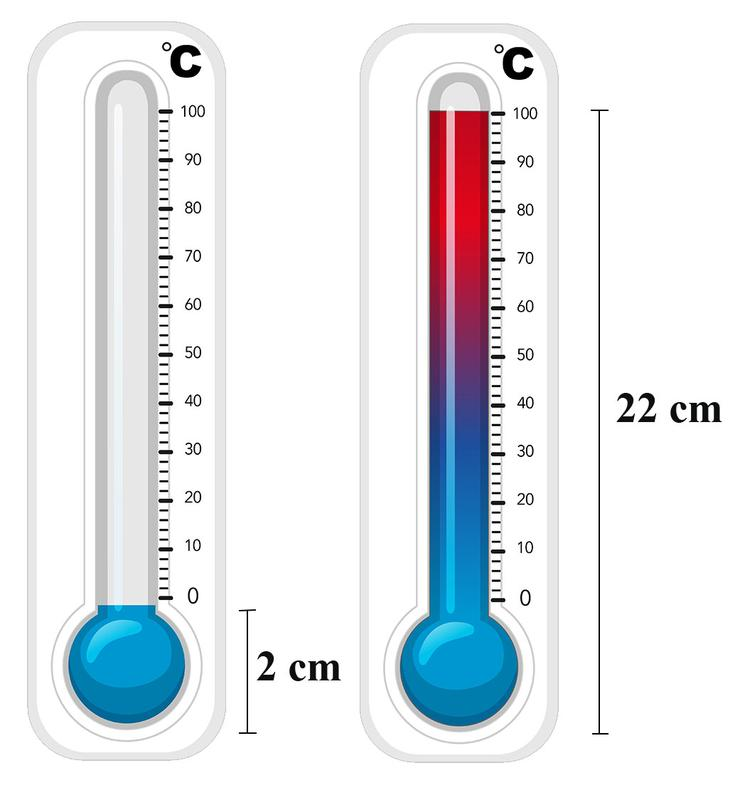
\includegraphics[width=4cm]{Images/nhietke22}}
	\loigiai{
		Chiều dài cột thủy ngân tỷ lệ với nhiệt độ. Do đó, ta có thể sử dụng phương pháp tỉ lệ để tìm nhiệt độ tương ứng.
		
		Xác định chiều dài cột thủy ngân tăng thêm cho mỗi độ Celsius:
		\[ L_{\Delta} = L_{100^\circ C} - L_{0^\circ C} = 22 \, \text{cm} - 2 \, \text{cm} = 20 \, \text{cm} \]
		
		Chiều dài cột thủy ngân tăng thêm tương ứng với một độ Celsius là:
		\[ \Delta L = \dfrac{20 \, \text{cm}}{100^\circ C} = 0.2 \, \text{cm/}^\circ C \]
		
		Chiều dài cột thủy ngân là $8 \, \text{cm}$, tức là chiều dài tăng thêm so với lúc $0^\circ C$ là:
		\[ L_{\text{tăng}} = 8 \, \text{cm} - 2 \, \text{cm} = 6 \, \text{cm} \]
		
		Vậy nhiệt độ tương ứng sẽ là:
		\[ T = \dfrac{L_{\text{tăng}}}{\Delta L} = \dfrac{6 \, \text{cm}}{0.2 \, \text{cm/}^\circ C} = 30^\circ C \]
		
		Vậy nhiệt độ khi chiều dài cột thủy ngân là $8 \, \text{cm}$ là $30^\circ C$.
	}
	\haidong{4}\end{vidu}
\begin{vidu}
	Một thước $cm$ được đặt dọc theo một nhiệt kế thủy ngân chưa được chia vạch như hình dưới đây. Trên
	nhiệt kế chỉ đánh dấu điểm đóng băng và điểm sôi của nước tinh khiết ở áp suất tiêu chuẩn. Giá trị nhiệt độ
	đang hiển thị trên nhiệt kế xấp xỉ là
	\begin{center}
		\begin{tikzpicture}[>=stealth',draw=Mapcolor, very thick, ]%nhiệt kế thủy ngân
			%\draw[dotted] (-2,-1) grid (14,2);
			\draw [rounded corners=0.2cm] (0.4,-0.25) rectangle (13,0.25);
			\draw [rounded corners=0.1cm] (-0.4,-0.1) rectangle (12.2,0.1);
			\draw [rounded corners=0.1cm, fill=Mapcolor!40] (-0.4,-0.1) rectangle (6.8,0.1);
			\foreach \x in {0,0.1,...,12}{
				\draw (\x,-0.3) -- (\x, -0.5);
			}
			\foreach \x in {0,...,12}{
				\draw (\x,-0.3) -- (\x,-0.7) node [below] {\x};
			}
			\draw (1,-0.3) -- (1,1) node [above] {Điểm đóng băng};
			\draw (12,-0.3) -- (12,1) node [above] {Điểm sôi};
			\draw (6.8,0) -- (6.8,1) node[above] {$6,8$};
		\end{tikzpicture}
	\end{center}
	\choice
	{$68^\circ C$}
	{$58^\circ C$}
	{$43^\circ C$}
	{\True $53^\circ C$}
	\loigiai{
		Ta có: $\dfrac{\Delta x}{\Delta t\left( ^\circ C\right)}  = \text{hằng số} \Rightarrow \dfrac{12-1}{100 - 0} = \dfrac{6,8-1}{t-0} \Rightarrow t \approx 52,72^\circ C$
	}
	
\end{vidu}

\begin{vidu}
	Để nhiệt kế nhạy hơn, người ta giảm đường kính tiết diện của ống chứa thủy ngân đi $2$ lần. Lúc này mỗi độ chia trong thang nhiệt độ Kelvin ứng với chiều dài bằng bao nhiêu $mm$ trên nhiệt kế mới?
	\shortans[oly]{$8$} 
	\loigiai{
		\begin{itemize}
			\item 
			\item 
		\end{itemize}
	}
\end{vidu}
\begin{vidu}
	\immini[thm]{Sự phụ thuộc vào nhiệt độ của bước sóng điện từ theo hệ thức Wien: $T .\lambda_{\max} = 2900\ \mu m .K$ được dùng vào việc chế tạo các nhiệt kế thường dùng hằng ngày như nhiệt kế hồng ngoại, cũng như các nhiệt kế trong thiên văn để đo nhiệt độ bề mặt của các thiên thể. Xét một nhiệt kế hồng ngoại khi đo nhiệt độ cơ thể người như hình vẽ. Bước sóng hồng ngoại do cơ thể người phát ra xấp xỉ bằng
		\choice
		{\True $9,4\ \mu m$}
		{$79\ \mu m$}
		{$29\ \mu m$}
		{$10,6\ \mu m$}}{
		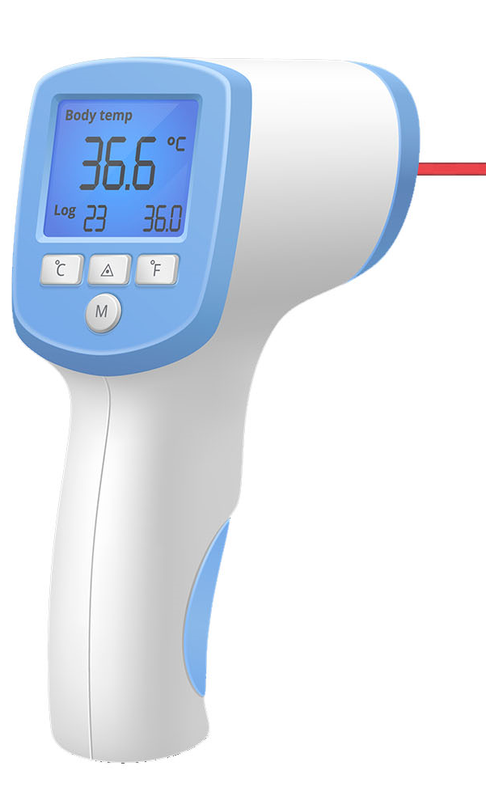
\includegraphics[width=2.5cm]{Images/tung123}
	}
	\loigiai{
		Sử dụng định luật dịch chuyển Wien:
		\[ T \cdot \lambda_{\max} = 2900\ \mu m \cdot K \]
		Trong đó, nhiệt độ trung bình của cơ thể người là khoảng $T = 310 \, \text{K}$.
		Tính bước sóng cực đại $\lambda_{\max}$:
		\[ \lambda_{\max} = \dfrac{2900 \, \mu m \cdot K}{310 \, \text{K}} \approx 9,35 \, \mu m \]
		Vậy, bước sóng hồng ngoại do cơ thể người phát ra xấp xỉ bằng $9,4 \, \mu m$.
	}
	\haidong{4}\end{vidu}

\begin{vidu}
	Một nhiệt kế khí thể tích không đổi hiển thị nhiệt độ $0^\circ C$ và $100^\circ C$ tương ứng với các áp suất $50\ cmHg$ và $90\ cmHg$. Biết nhiệt độ đọc được là hàm bậc nhất của áp suất. Khi áp suất thủy ngân là $60\ cmHg$ thì nhiệt độ đọc được là
	\choice
	{\True $25^\circ C$}
	{$40^\circ C$}
	{$15^\circ C$}
	{$12,5^\circ C$}
	\loigiai{
		Nhiệt độ và áp suất có mối quan hệ tuyến tính theo dạng hàm bậc nhất:
		\[ T = aP + b \]
		
		Dùng hai điểm chuẩn ($P_1, T_1$) và ($P_2, T_2$) để lập phương trình:\\
		Với $T_1 = 0^\circ C$ ở $P_1 = 50 \, \text{cmHg}$:
		\[ 0 = a \cdot 50 + b \]
		
		Với $T_2 = 100^\circ C$ ở $P_2 = 90 \, \text{cmHg}$:
		\[ 100 = a \cdot 90 + b \]
		
		Giải hệ phương trình này, ta có:
		\[ b = -50a \]
		\[ 100 = 90a - 50a \]
		\[ 100 = 40a \]
		\[ a = 2,5 \]
		\[ b = -50 \times 2,5 = -125 \]
		
		Vậy, phương trình nhiệt độ theo áp suất là:
		\[ T = 2,5 P - 125 \]
		
		Khi áp suất là $60 \, \text{cmHg}$, nhiệt độ là:
		\[ T = 2,5 \times 60 - 125 = 150 - 125 = 25^\circ C \]
	}
	\haidong{4}\end{vidu}

\begin{vidu} \nguon{2}
	Trong phạm vi từ $0^\circ C$ đến $600^\circ C$ thì điện trở của một dây platin (bạch kim) phụ thuộc vào nhiệt độ theo hệ thức: $R=10\left(1+2 t+4 t^2\right)$ (t đo bằng $^\circ C$, R đo bằng $\Omega$). Nếu điện trở của dây bạch kim bằng $4210\ \Omega$ thì nhiệt độ của dây bạch kim bằng
	\choice
	{$4210 \ K$}
	{\True $10^\circ C$}
	{$610^\circ C$}
	{$610 \ K$}
	\loigiai{
		Từ: $R=10\left(1+2 t+4 t^2\right)=4210 \Rightarrow t=10^\circ C $ 
	}
\end{vidu}

\loai{Loại 6: Thang nhiệt độ giả sử}
\begin{vidu}
	Một thang đo $X$ lấy điểm băng là $-10 X$, lấy điểm sôi là $90 X$. Biết mỗi độ X bằng $\dfrac{1}{100}$ khoảng cách giữa điểm băng và điểm sôi. Nhiệt độ của một vật đọc được trên nhiệt kế Celsius là $40^\circ C$ thì trên thang đo $X$ có nhiệt độ bằng
	\choice
	{$20 X$}
	{\True $30 X$}
	{$40 X$}
	{$50 X$}
	\loigiai{
		Khoảng cách giữa điểm băng và điểm sôi trên thang đo X là:
		\[ 90X - (-10X) = 100X \]
		
		Mỗi độ X tương ứng với:
		\[ \text{Mỗi độ X} = \dfrac{100^\circ C}{100 X} = 1^\circ C \]
		
		Nhiệt độ $40^\circ C$ trên thang Celsius tương ứng với:
		\[ 40 X + (-10 X) = 40 - 10 = 30 X \]
		
		Vậy nhiệt độ đọc được trên thang đo $X$ là $30 X$.
	}
	\haidong{4}\end{vidu}

\begin{vidu} \nguon{4}
	Có hai thang đo nhiệt độ $X$ và $Y$ liên hệ với nhau theo công thức $T_{X}=\dfrac{3}{4} \ T_{Y}+20$. Độ biến thiên nhiệt độ $30^\circ X$ trong thang nhiệt $X$ sẽ tương ứng với một độ biến thiên trong thang nhiệt $Y$ là
	\choice
	{$66,6^\circ Y$}
	{\True $40^\circ Y$}
	{$60^\circ Y$}
	{$86,6^\circ Y$}\loigiai{
		Độ biến thiên $30^\circ X$ sẽ tương ứng với độ biến thiên trong thang nhiệt $Y$ là:
		$$
		\Delta T_{Y}=30 . \dfrac{4}{3}=40^\circ Y
		$$
	}
\end{vidu}
 \begin{vidu} \nguon{2}
 	Giả sử một học sinh tạo ra một nhiệt kế sử dụng một thang nhiệt độ mới cho riêng mình, gọi là nhiệt độ $Z$, có đơn vị là ${}^\circ Z$. Trong đó nhiệt độ của nước đá đang tan ở $1\ atm$ là $-5^\circ Z$, nhiệt độ nước đang sôi ở $1\ atm$ là $105^\circ Z$ và mỗi độ $Z$ là $\dfrac{1}{110}$ của khoảng hai nhiệt độ này.
 	\begin{vdc}
 		Biểu thức chuyển đổi giữa nhiệt độ Celsius và độ $Z$ là
 		\choice
 		{$t\ (^\circ Z) = 0,9.t\ (^\circ C) - 5$}
 		{\True $t\ (^\circ Z) = 1,1.t\ (^\circ C) - 5$}
 		{$t\ (^\circ Z) = 1,1.t\ (^\circ C) + 5$}
 		{$t\ (^\circ Z) = 1,1. t\ (^\circ C) - 5$}
% 		\loigiai{
% 			\begin{itemize}
% 				\item[A] Sai: Dùng sai hệ số chuyển đổi, hệ số đúng là $1,1$
% 				\item[B] Đúng: $t\ (^\circ Z) = 1,1t\ (^\circ C) - 5$ từ khoảng $110^\circ Z$ ứng với $100^\circ C$
% 				\item[C] Sai: Dấu cộng sai, làm lệch toàn bộ biểu thức
% 				\item[D] Sai: Dạng phân phối sai cấu trúc biểu thức
% 			\end{itemize}
% 		}

 	\end{vdc}
 	\dotlineEX{4}
 	\begin{vdc}
 		Nếu nhiệt kế chỉ $61^\circ Z$, thì nhiệt độ của vật theo Celsius là
 		\choice
 		{$55^\circ C$}
 		{$61^\circ C$}
 		{\True $60^\circ C$}
 		{$50^\circ C$}
% 		\loigiai{
% 			\begin{itemize}
% 				\item[A] Sai: Tính ngược sai từ biểu thức chuyển đổi
% 				\item[B] Sai: Nhầm số chỉ giữa hai thang
% 				\item[C] Đúng: $61 = 1,1t - 5 \Rightarrow t = 60^\circ C$
% 				\item[D] Sai: Nhầm phương trình khi thế ngược
% 			\end{itemize}
% 		}

 	\end{vdc}
 	\dotlineEX{4}
 	\begin{vdc}
 		Nhiệt độ nào (theo Celsius) khiến số chỉ trên cả hai thang đo bằng nhau?
 		\choice
 		{$60^\circ C$}
 		{$61^\circ C$}
 		{$55^\circ C$}
 		{\True $50^\circ C$}
% 		\loigiai{
% 			\begin{itemize}
% 				\item[A] Sai: $t\ (^\circ Z)$ và $t\ (^\circ C)$ không bằng nhau tại $60^\circ C$
% 				\item[B] Sai: Lý luận sai khi thế vào biểu thức chuyển đổi
% 				\item[C] Sai: Chỉ gần đúng, không đúng nghiệm phương trình
% 				\item[D] Đúng: $t = 1,1t - 5 \Rightarrow t = 50^\circ C$
% 			\end{itemize}
% 		}

 	\end{vdc}
	\dotlineEX{4}
 \end{vidu}
 

\begin{vidu} \nguon{4}
	Một thang đo nhiệt độ Y, trong đó nhiệt độ nước đá đang tan ở 1 atm là  $-25^\circ Y$, nhiệt độ sôi của nước ở 1 atm là $85^\circ Y$ và mỗi độ Y là $\dfrac{1}{110}$ của khoảng hai nhiệt độ này. Nhiệt độ $70^\circ Y$ xấp xỉ bằng bao nhiêu độ Kelvin?
	\choice
	{\True $360 \ K$}
	{$377 \ K$}
	{$350 \ K$}
	{$366 \ K$}\loigiai{
		
		Độ biến thiên $110^\circ Y$ tương ứng với độ biến thiên $100 \ K$.
		
		Vậy độ biến thiên $95^\circ Y$ tương ứng với độ biến thiên $86,36 \ K$.
		
		Nhiệt độ $70^\circ Y$ sẽ tương ứng với nhiệt độ trong thang nhiệt Kelvin là:
		$$
		T=273,16+86,36\approx 360 \ K
		$$
	}
\end{vidu}
\begin{vidu}
	Biết rằng mối liên hệ giữa các giá trị nhiệt độ trên hai thang đo nhiệt độ Fahrenheit $t\ (^\circ F)$ và Celsius $t\ (^\circ C)$ được cho bởi công thức $t\ (^\circ F)=32+1,8t\ (^\circ C)$. Giả sử có một thang nhiệt độ kí hiệu là Z. Ở áp suất 1 atm, nhiệt độ sôi của nước theo thang này là $60 Z$, nhiệt độ đóng băng của nước là $-15 Z$ và mỗi độ Z là $\dfrac{1}{75}$ của khoảng hai nhiệt độ này. Nhiệt độ của vật theo thang Fahrenheit là bao nhiêu nếu thang $Z$ là $-96 Z$?
	\choice
	{$-62,4^\circ F$}
	{$162,4^\circ F$}
	{\True $-162,4^\circ F$}
	{$62,4^\circ F$}
	\loigiai{		
		Tìm khoảng cách nhiệt kế:
		\[ \Delta Z = 60 Z - (-15 Z) = 75 Z \]
		\[ \Delta^\circ C = 100^\circ C - 0^\circ C = 100^\circ C \]
		
		$1^\circ C$ tương ứng với:
		\[ \dfrac{75}{100}Z = \dfrac{3}{4}Z\]
		
		Tìm nhiệt độ theo $^\circ C$ tương ứng với $-96 Z$:
		\[ T_{\textsubscript{C}} = \dfrac{-96 Z + 15 Z}{\dfrac{75 Z}{100^\circ C}} = \dfrac{81}{3/4} = -108^\circ C \]
		
		Chuyển $T_{\textsubscript{C}}$ sang $^\circ F$:
		\[ T_{\textsubscript{F}} = (32 + 1.8 T_{\textsubscript{C}}) \approx -162,4^\circ F \]
	}
	\haidong{4}\end{vidu}
